
%----------------------------------------------------------------------------------------------------------------------------------------

% définit le type de document et ses options
\documentclass[a4paper,10pt]{article}

% des paquetages indispensables, qui ajoutent des fonctionnalites
\usepackage[utf8]{inputenc}
\usepackage{graphicx}
\usepackage{lscape}
\usepackage{url}
\usepackage{xspace}
\usepackage[francais]{babel}
%\usepackage{fullpage}

\pagestyle{plain}


%----------------------------------------------------------------------------------------------------------------------------------------


% le debut du contenu
\begin{document}


%----------------------------------------------------------------------------------------------------------------------------------------


%%%%%%%%%%%%%%%%%%%%%%%%%%%%%%%%%%%%%%%%%%%%%%%%%
%%Page d'accueil
\begin{center}
	%%
	\hspace{3cm}
	
\includegraphics[scale=0.8]{logo.ps}

	%%
	\vspace{1cm}
	{\large Projet de spécialité 2010}\\
	{\Large Conception d'un modèle de feu 3D temps réel}\\
	\vspace{1cm}


	\includegraphics[scale=0.3]{feu.ps}\\
	\vspace{2cm}
	%%
	Etudiants impliqués :\\
	Benjamin Aupetit - IRVM - benjamin.aupetit@ensimag.imag.fr\\
	Julien Champeau - IRVM - julien.champeau@ensimag.imag.fr\\
	Arnaud Emilien - IRVM - arnaud.emilien@ensimag.imag.fr\\
	~\\
	Encadrants :\\
	Marie-Paule Cani  -  Marie-Paule.Cani@inrialpes.fr \\
	Aurélie Catel - aurelie.catel@grenoble-inp.fr
	~ \\
	\vspace{3mm}
	Ensimag 2010\\

\end{center}

\newpage

\tableofcontents

\newpage



%----------------------------------------------------------------------------------------------------------------------------------------
%%%%%%%%%%%%%%%%%
\section{Présentation du projet}
\subsection{Introduction}

\subsection{Objectifs}


\subsection{Aperçu}


\subsection{Analyses Bibliographiques}
%%%%%%%%%%%%%%%%%
Cette section regroupe les différents articles lus, concernant les travaux déjà effectués dans ce domaine. 
Nous allons expliquer brièvement de quoi ils parlent, ce que nous en avons retenu de bien ou de mal, ce que nous allons 
utiliser...

\subsubsection{Real-Time Fluid Dynamics for Games}
\textbf{Auteurs} : Jos Stam.\\
\textbf{Publication} : \\
\textbf{Sujet(s) abordé(s)} : \\
\textbf{Point(s) positif(s)} :\\
\textbf{Point(s) négatif(s)} :\\
\textbf{Conclusion} :\\

\subsubsection{Stable Fluids}
\textbf{Auteurs} : Jos Stam.\\
\textbf{Publication} :\\
\textbf{Sujet(s) abordé(s)} : \\
\textbf{Point(s) positif(s)} :\\
\textbf{Point(s) négatif(s)} :\\
\textbf{Conclusion} :\\


\subsubsection{An Interactive Simulation Framework for Burning Objets}
\textbf{Auteurs} : Zeki Melek, John Keyser.\\
\textbf{Publication} :\\
\textbf{Sujet(s) abordé(s)} : \\
\textbf{Point(s) positif(s)} :\\
\textbf{Point(s) négatif(s)} :\\
\textbf{Conclusion} :\\


\subsubsection{Visual Simulation of Smoke}
\textbf{Auteurs} : Ronald Fedkiw, Jos Stam, Henrik Wann Jensen.\\
\textbf{Publication} :\\
\textbf{Sujet(s) abordé(s)} : \\
\textbf{Point(s) positif(s)} :\\
\textbf{Point(s) négatif(s)} :\\
\textbf{Conclusion} :\\

\subsubsection{Simulating Water and Smoke with an Octree Data Structure}
\textbf{Auteurs} : Frank Losasso, Frédéric Gibou, Ron Fedkiw.\\
\textbf{Publication} :\\
\textbf{Sujet(s) abordé(s)} : \\
\textbf{Point(s) positif(s)} :\\
\textbf{Point(s) négatif(s)} :\\
\textbf{Conclusion} :\\



\subsubsection{Real-Time Simulation of Deformation and Fracture of Stiff Materials}
\textbf{Auteurs} : Matthias Müller, Leonard McMillan, Julie Dorsey, Robert Jagnow.\\
\textbf{Publication} :\\
\textbf{Sujet(s) abordé(s)} : \\
\textbf{Point(s) positif(s)} :\\
\textbf{Point(s) négatif(s)} :\\
\textbf{Conclusion} :\\



\subsubsection{Voxels On Fire}
\textbf{Auteurs} : Ye Zhao, Xiaoming Wei, Zhe Fan, Arie Kaufman, Hong Qin.\\
\textbf{Publication} :\\
\textbf{Sujet(s) abordé(s)} : \\
\textbf{Point(s) positif(s)} :\\
\textbf{Point(s) négatif(s)} :\\
\textbf{Conclusion} :\\

\subsubsection{Meshes On Fire}
\textbf{Auteurs} : Haeyoung Lee, Laehyun, Mark Meyer, Mathieu Desbrun.\\
\textbf{Publication} :\\
\textbf{Sujet(s) abordé(s)} : Propagation des flammes à la surface d'un objet.\\
\textbf{Point(s) positif(s)} :\\
\textbf{Point(s) négatif(s)} :\\
\textbf{Conclusion} :\\

\subsubsection{Real-time Procedural Volumetric Fire}
\textbf{Auteurs} : Alfred R. Fuller, Hari Krishnan, Karim Mahrous, Bernd Hamann, Kenneth I. Joy.\\
\textbf{Publication} :\\
\textbf{Sujet(s) abordé(s)} : \\
\textbf{Point(s) positif(s)} :\\
\textbf{Point(s) négatif(s)} :\\
\textbf{Conclusion} :\\



%----------------------------------------------------------------------------------------------------------------------------------------
%%%%%%%%%%%%%%%%%
\section{Mise en place du modèle global}
%%%%%%%%%%%%%%%%%




%----------------------------------------------------------------------------------------------------------------------------------------
%%%%%%%%%%%%%%%%%
\section{Modèle de flamme}
%%%%%%%%%%%%%%%%%





%----------------------------------------------------------------------------------------------------------------------------------------
%%%%%%%%%%%%%%%%%
\section{Modèle de fumée}
%%%%%%%%%%%%%%%%%





%----------------------------------------------------------------------------------------------------------------------------------------
%%%%%%%%%%%%%%%%%
\section{Propagation sur l'objet}
%%%%%%%%%%%%%%%%%





%----------------------------------------------------------------------------------------------------------------------------------------
%%%%%%%%%%%%%%%%%
\section{Destruction de l'objet}
%%%%%%%%%%%%%%%%%





%----------------------------------------------------------------------------------------------------------------------------------------
%%%%%%%%%%%%%%%%%
\section{Propagation dans l'environnement}
%%%%%%%%%%%%%%%%%


%----------------------------------------------------------------------------------------------------------------------------------------
%%%%%%%%%%%%%%%%%
\section{Références}
%%%%%%%%%%%%%%%%%


%----------------------------------------------------------------------------------------------------------------------------------------
\end{document}
